\documentclass[11pt]{utalcaDoc}
\usepackage{alltt}
\usepackage{underscore}
\usepackage[utf8]{inputenc}
\usepackage[activeacute,spanish]{babel}
\usepackage{verbatim}
\usepackage[pdftex]{graphicx}
\usepackage{epstopdf}
\usepackage{ae}
\usepackage{bigfoot}
\usepackage{enumerate}
\usepackage{amsmath}
\usepackage{amsfonts}
\usepackage{algorithm}
\usepackage{imakeidx}
\usepackage{algorithmic}
\usepackage{hyperref}



\title{{\bf Gestion de Redes}\\Laboratorio 4\\Ripv2 y RIPng}
\author{
    \bf{Profesor:} José Letelier (\texttt{jletelier@utalca.cl})\\ 
    \bf{Alumno Ayudante:} Erik Regla (\texttt{eregla09@alumnos.utalca.cl})\\ }
\date{\today}

\makeindex[columns=3, title=Alphabetical Index, intoc]
\begin{document}
\renewcommand{\figurename}{Figura~}
\renewcommand{\tablename}{Tabla~}

\maketitle
%\newpage
%\tableofcontents

%\newpage
\section{Descripción}
En este laboratorio se espera que el alumno se familiarize con los mecanismos de ruteo RIP para los protocolos IPv4 e IPv6.

\section{Actividad a desarrollar}

A continuación se presenta una red consistente de tres enrutadores, de la cual se espera que se implemente RIP y posteriormente realice las siguientes actividades.

\begin{figure}[!ht]
  \centering
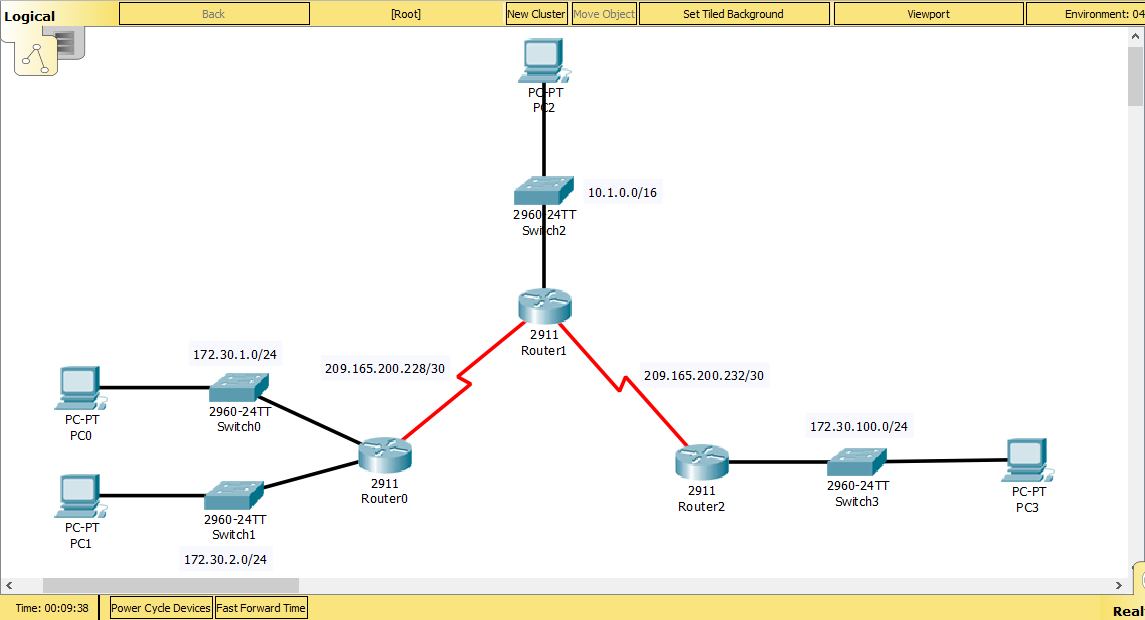
\includegraphics[scale=.3]{ipv4} 
  \caption{Diagrama IPv4}
  \label{FIGURE:1}
\end{figure}

\begin{figure}[!ht]
  \centering
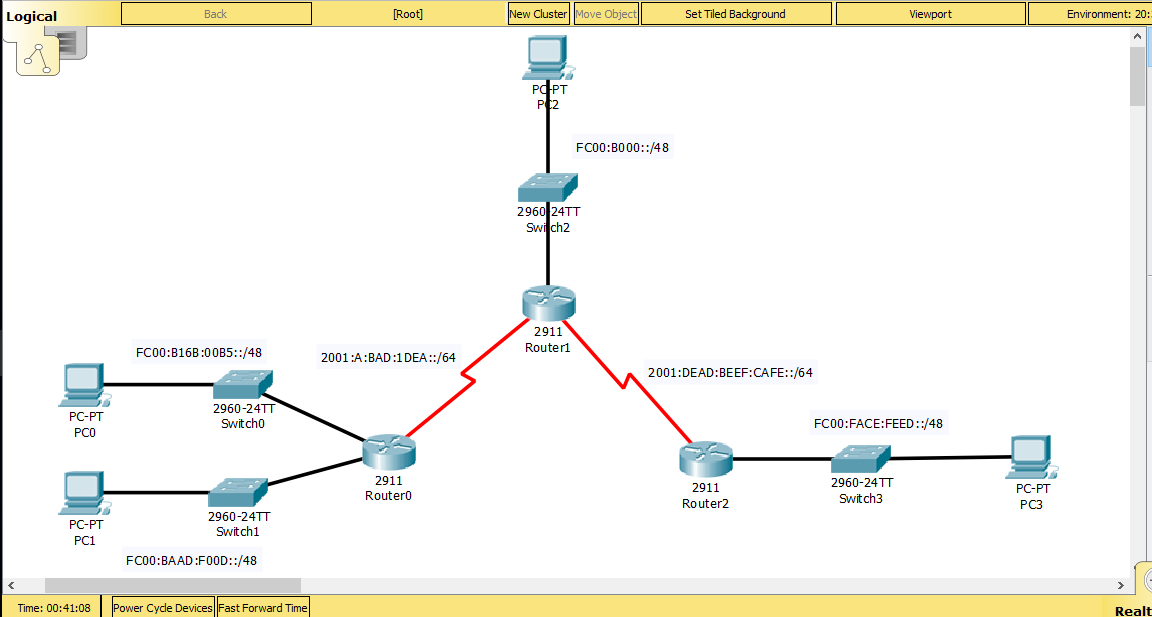
\includegraphics[scale=.3]{ipv6} 
  \caption{Diagrama IPv6}
  \label{FIGURE:2}
\end{figure}

\subsection{RIPv1}
\begin{enumerate}
  \item {Implemente el diagrama de la Figura \ref{FIGURE:1}.}
  \item {Examine el estado de la red para cada uno de los tres enrutadores (utilize el comando \texttt{show ip interface brief}).}
  \item {Realice pruebas de conectividad para los distintos equipos en la red e indique porcentaje de éxito:
    \begin{itemize}
      \item {PC1 a PC0}
      \item {PC2 a PC0}
      \item {PC3 a PC0}
      \item {PC1 a PC3}
      \item {PC2 a PC3}
    \end{itemize}
  }
  \item Examine las actualizaciones RIP propagadas.
  \item Indique la razón por la cual hay problemas de conectividad en la red.
\end{enumerate}

\subsection{RIPv2}
\begin{enumerate}
  \item{Cambie el protocolo de RIPv1 a RIPv2 y verifique que este se esté ejecutando.}
  \item Examine las actualizaciones RIP propagadas y liste sus rutas.
  \item Deshabilite la sumarización de rutas, examine las actualizaciones RIP propagadas, liste sus rutas e indique las diferencias con la version sumarizada.
  \item {Realice pruebas de conectividad para los distintos equipos en la red e indique porcentaje de éxito:
    \begin{itemize}
      \item {PC1 a PC0}
      \item {PC2 a PC0}
      \item {PC3 a PC0}
      \item {PC1 a PC3}
      \item {PC2 a PC3}
    \end{itemize}
  }
  \item Indique la razón por la cual ahora no hay problemas de conectividad en la red.
\end{enumerate}


\subsection{RIPng}
\begin{enumerate}
  \item {Implemente el diagrama de la Figura \ref{FIGURE:2}.}
  \item Examine las actualizaciones RIP propagadas y liste sus rutas.
  \item Habilite la sumarización de rutas, examine las actualizaciones RIP propagadas, liste sus rutas e indique las diferencias con la version sumarizada.
  \item Muestre las tablas de enrutamiento de cada uno de los enrutadores.
  \item Indique como podría replicar los problemas observados en el ejercicio de RIPv1.
\end{enumerate}





\section{Evaluación}
\begin{itemize}
  \item{RIPv1 \textbf{2.0 pto}}
  \item{RIPv2 \textbf{2.0 pto}}
  \item{RIPng \textbf{2.0 pto}}
\end{itemize}

\end{document}
